\documentclass[11]{article}
\usepackage[utf8]{inputenc}
\usepackage{graphicx}
\usepackage{subfig}
\usepackage[margin=0.25 in]{geometry}


 
\title{CMSC6950 PROJECT: 
Determining trends in a data set: An Application of pyMannKendall}
\author{SYLVIA ANKAMAH}
\date{August, 2020}
\graphicspath{}

\begin{document}
\maketitle
\section{Introduction}
The determination of trend in data sets gathered over time is important in decision making. Various tools are applicable in determining trends in a data set. However, the use of these tools depends on the distribution of the data set. One test that does not depend on the distribution of the data set is the Mann Kendall Trend test.\\Mannkendall Trend test(sometimes called the M-K test) is used to analyse data collected over time for consistently increasing or decreasing trends(monotonic). It is a non-parametric test which implies it works for all distribution.That is, it is not important for the data set to follow a specific distribution. However, there should not be serial correlation in the data. Minimum order of measurement for the MannKendall trend test is at least eight to ten. \\
The null hypothesis for the test is: there is no monotonic trend in the series.\\
The alternative hypothesis for the test is: a trend exists. The trend can be positive or negative.\\
pyMannKendall is a pure Python implementation of non-parametric Mann-Kendall trend analysis, which brings together almost all types of Mann-Kendall Test. Currently, this package has 11 Mann-Kendall Tests and 2 sen's slope estimator function. Brief description of three of the functions are below:\\
1. Original Mann-Kendall test (original test): Original Mann-Kendall test is a non-parametric test, which does not consider serial correlation or seasonal effects.\\
2. Hamed and Rao Modified MK Test (hamed rao modification test): This modified MK test was proposed by Hamed and Rao (1998) to address serial auto-correlation issues. They suggested a variance correction approach to improve trend analysis. User can consider first n significant lag by inserting lag number in this function. By default, it considered all significant lags.\\
3. Yue and Wang Modified MK Test (yue wang modification test): This is also a variance correction method for considered serial auto-correlation proposed by Yue and  Wang (2004). User can also set their desired significant n lags for the calculation.\\
This project aims to discuss how the pyMannKendall which is a python package can be used to determine trends in a data set. Three different ddata sets were used in this project so as to describe the usage of the pyMannKendall.\\


\section{Data description and Analysis}
\subsection{Data description}
Three various data sets were used in the analysis.The data sets are secondary data based on number of female births, sales of shampoo and malaria cases. The first data set is based on the daily total female births from the 1st of January, 1959 to the 31st of December, 1959. All three data sets were gathered on monthly basis. Also, the second data set, based on the shampoo sales were gathered over a three year period whiles the third data set, based on recorded Malaria data in the Ashanti region in Ghana, Africa, were based on the period, January, 2010 to December, 2014. There were no missing values in the data sets.Two of the data sets which includes daily total female births and shampoo sales were provided by Hussain et al., (2019).
\subsection{Analysis}
\subsubsection{Female births}
From the summary statistics, the mean number of births was 41.98 with a minimum value of 23 and a maximum value of 73. The total births over the study period was 365. Adescriptive plot was obtained and shown in Figure 1. 
\begin{figure}%
	    \centering
	    \subfloat[TREND PLOT FOR BIRTHS]{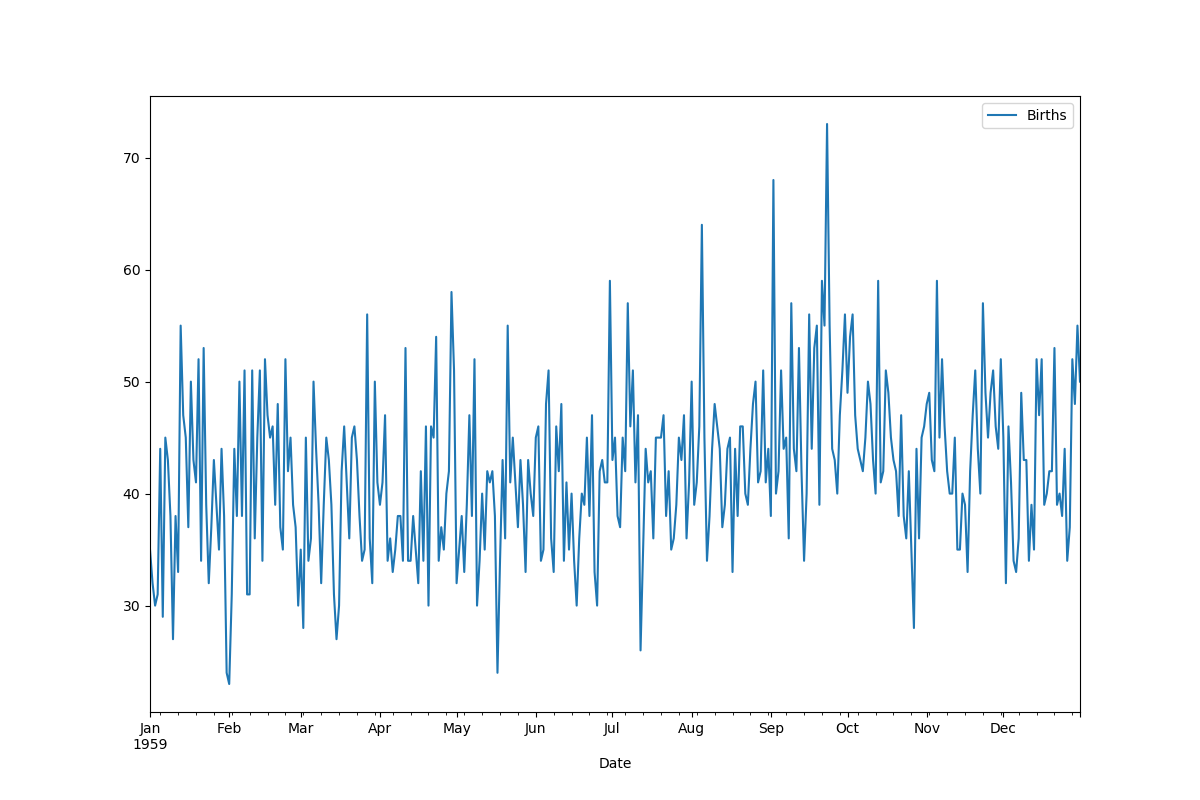
\includegraphics[scale=0.3]{Birth_data_Trend_plot.png}}%
	    \qquad
	    \subfloat[AUTO-CORRELATION PLOT FOR BIRTHS]{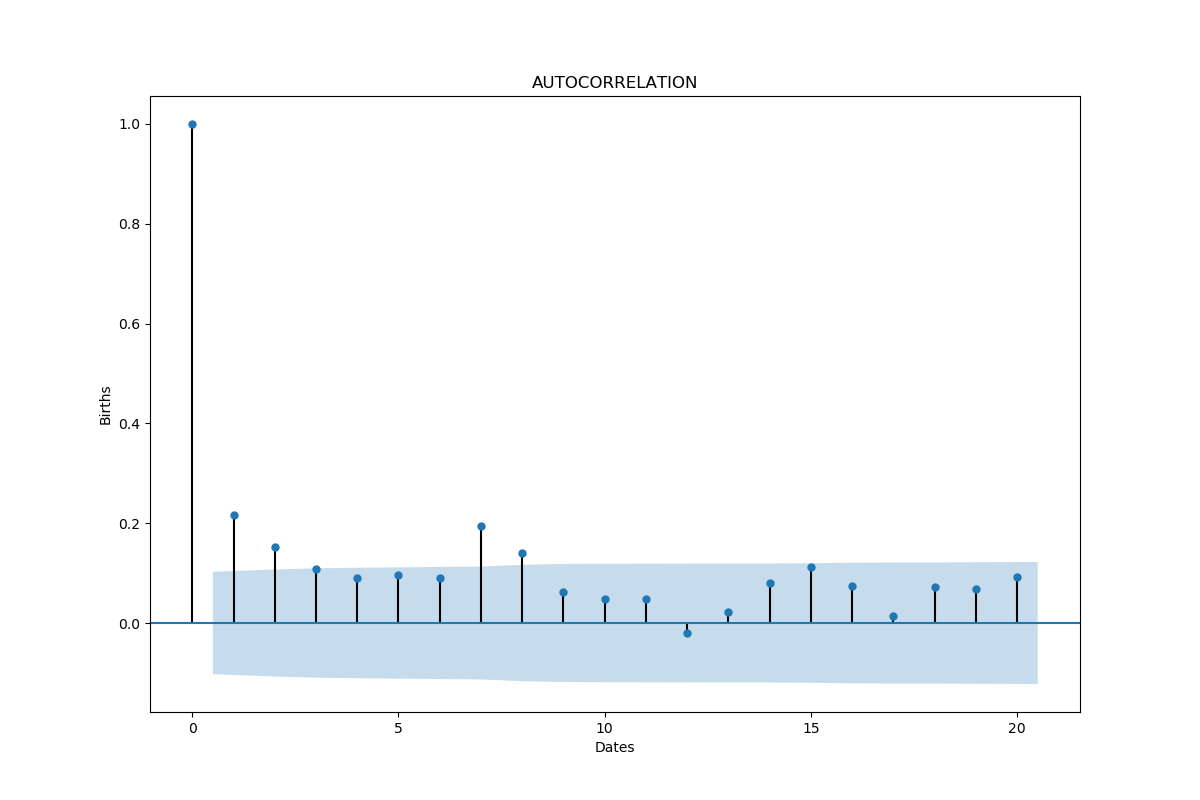
\includegraphics[scale=0.3]{BIRTH_DATA_ACF_PLOT.png}}%
	    \qquad
	    \subfloat[TRENDLINE PLOT FOR BIRTHS]{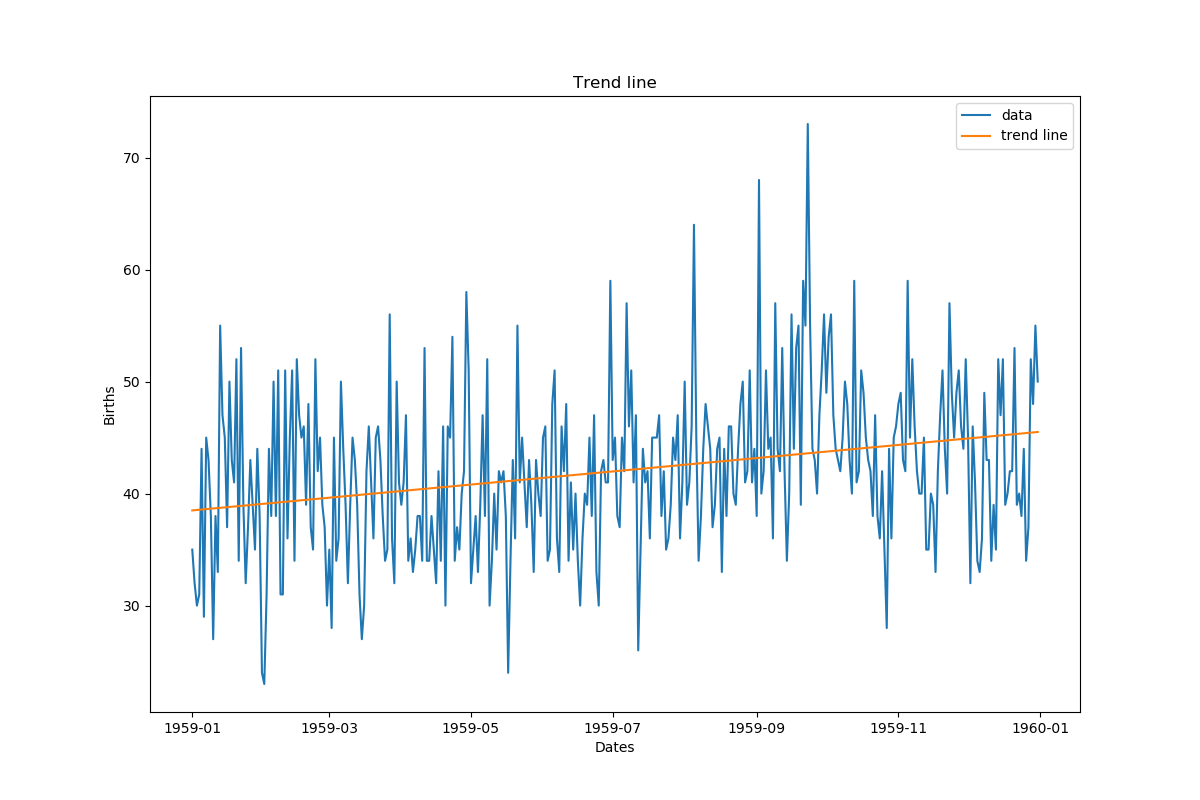
\includegraphics[scale=0.3]{Birth_data_Trendline.png}}
		    \caption{PLOTS FOR BIRTH DATA}
		        \label{fig:1}
\end{figure}
Further, an  autocorrelation plot was obtained and also shown in Figure 1. This plot is to help determine whether there are correlations in the data set and this would further inform the type of test pyMannkendall test to use. From the plot, it can be observed that there is a slight autocorrelation at lag 1 and as such, it was assumed that there is no correlation in the data set.                                                                                    
Based on results obtained from the ACF plot, the Original Mann Kendall test was used to test the trend.\\The output from the Original MannKendall trend test indicates there is a trend(increasing) in the data set with a p-value of 1.144585e-07 which is lesser than 0.05. Therefore, the null hypothesis is rejected indicating there is a trend in the data set.\\ Further, the original data set was plotted together with the trend line indicating the direction and this is shown in Figure 1.
\subsubsection{Shampoo data}
From the sales of shampoo data set, the minimum value of number of shampoo sold over the three year period was 119.3 and the maximum number was 682 with a mean value of 312.6.\\ A descriptive plot is shown in Figure 2.\\ Further, an Autocorrelation plot is shown in Figure 2. The Auto-correlation plot indicates that there is autocorrelation in the first lag. Therefore, a modified MannKendall test must be used. In this report, three tests were used but only one would be discussed, which is the Hamed and Rao Modified Mk test.
\begin{figure}%
	    \centering
	    \subfloat[TREND PLOT FOR SHAMPOO SALES]{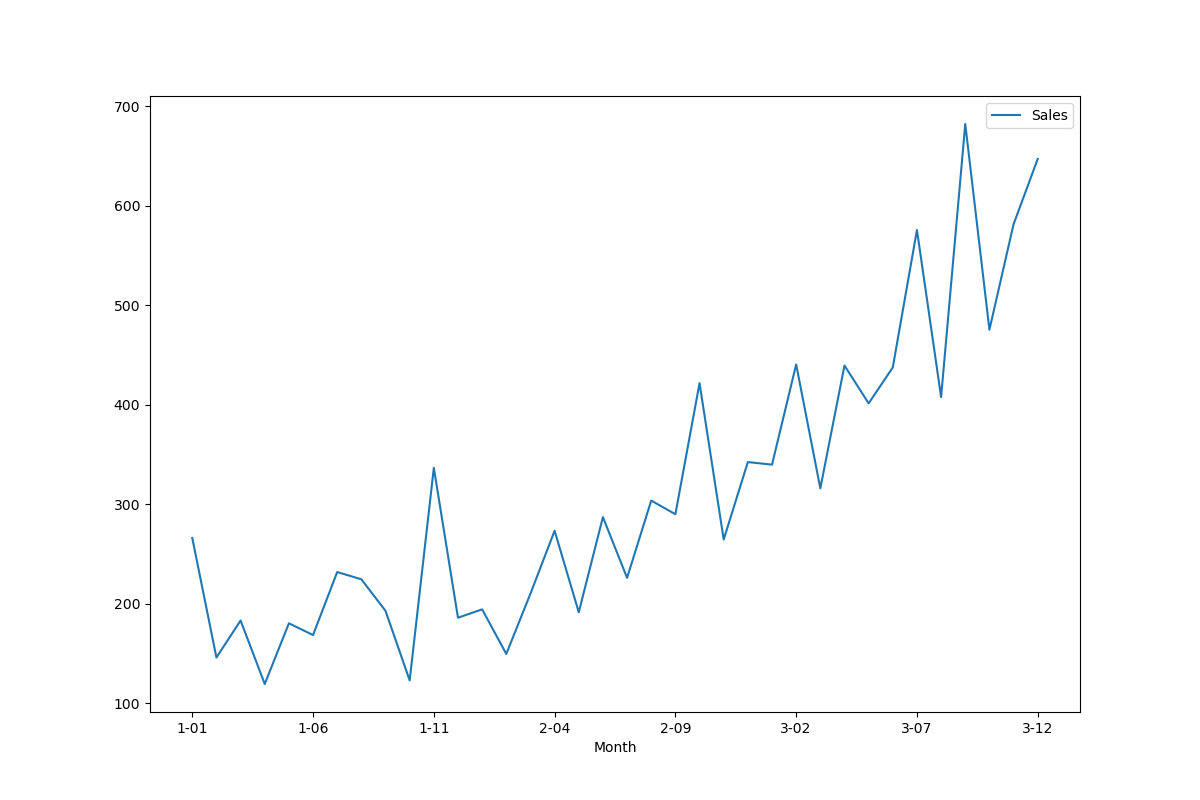
\includegraphics[scale=0.3]{Shampoo_data_Trend_plot.png}}%
	    \qquad                                                                                                                  \subfloat[AUTO-CORRELATION PLOT FOR SHAMPOO SALES]{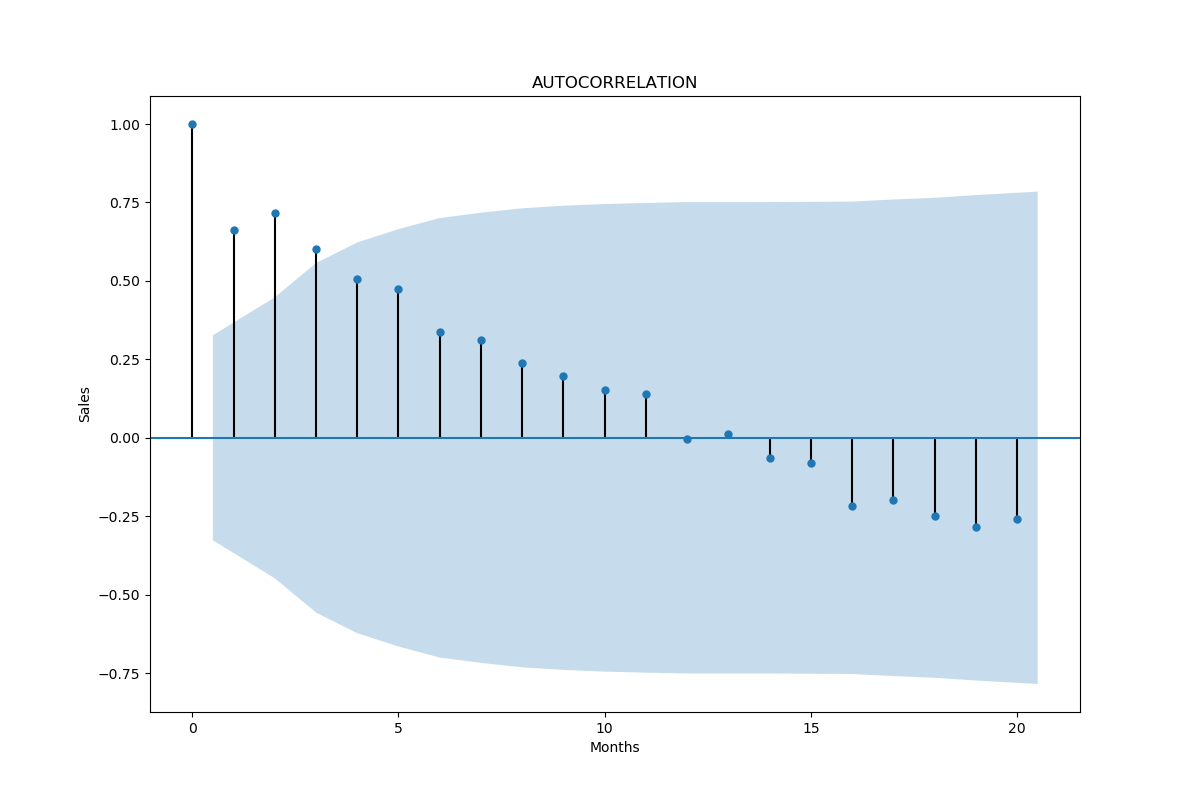
\includegraphics[scale=0.3]{SHAMPOO_DATA_ACF_PLOT.png}}%
	    \qquad                                                                                                                  \subfloat[TRENDLINE PLOT FOR SHAMPOO SALES]{\includegraphics[scale=0.3]{SHAMPOO_DATA_Trendline.png}}                            \caption{PLOTS FOR SHAMPOO DATA}                                                                                             \label{fig:2}
\end{figure}
Based on results obtained from the ACF, a modified MannKendall test must be used. In this report, three tests were used but only one would be discussed, which is the Hamed and Rao Modified Mk test. 
The output obtained from the Hamed and Rao Modified Mk test indicates that there is an increasing trend with a p-value of 2.8196e-07(the null hypothesis is rejected).\\ For the other tests not shown here, similar results were obtained. That is Yue and Wang Modified MK Test (yue wang modification test) and Modified MK test using Trend free Pre-Whitening method (trend free pre whitening modification test)\\A third plot indicating the direction of the trend is also shown in Figure 2.\\
\subsubsection{Malaria Data}
From the malaria data spanning over a five year period, the minimum number of monthly recorded malaria cases was 36047 and the maximum value was 87765. The mean value was 65317.96. \\ The descriptive and Auto-correlation plots are shown in Figure 3.
\begin{figure}%
	    \centering
	    \subfloat[TREND PLOT FOR MALARIA DATA]{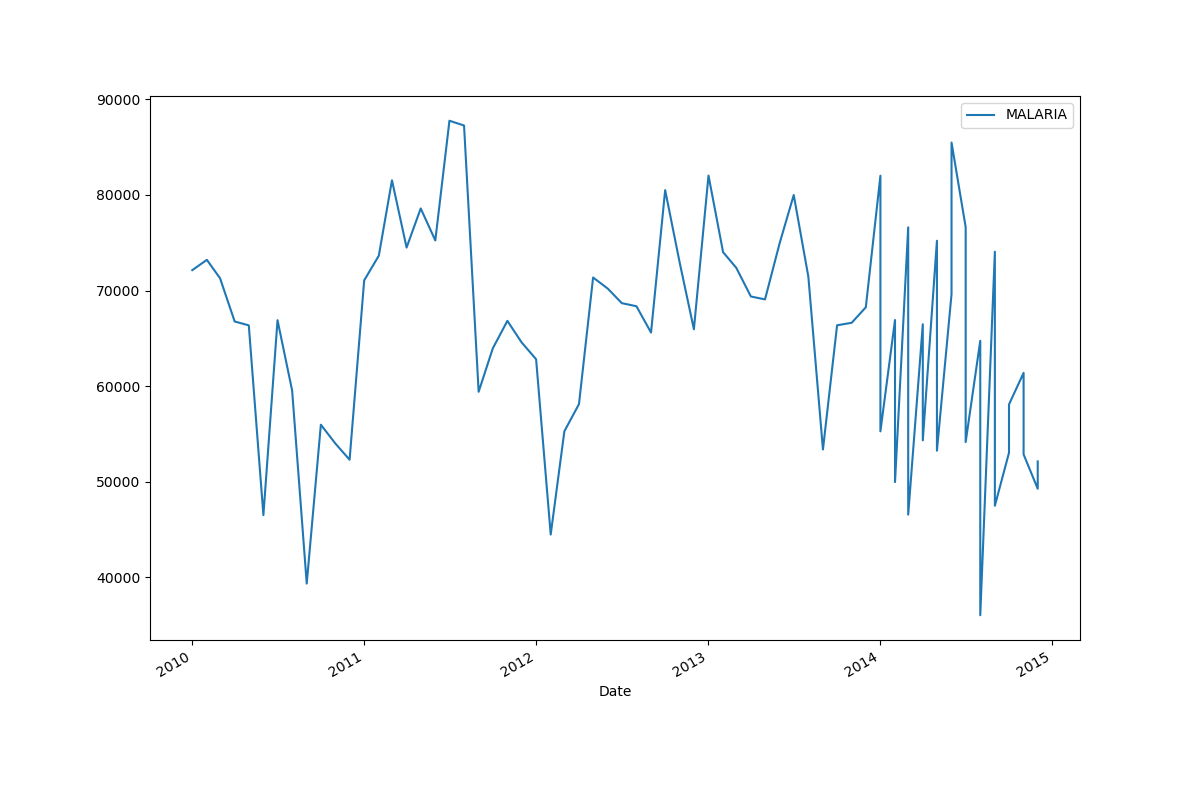
\includegraphics[scale=0.3]{Malaria_Trend_plot.png}}%
	    \qquad
	    \subfloat[AUTO-CORRELATION PLOT FOR MALARIA DATA]{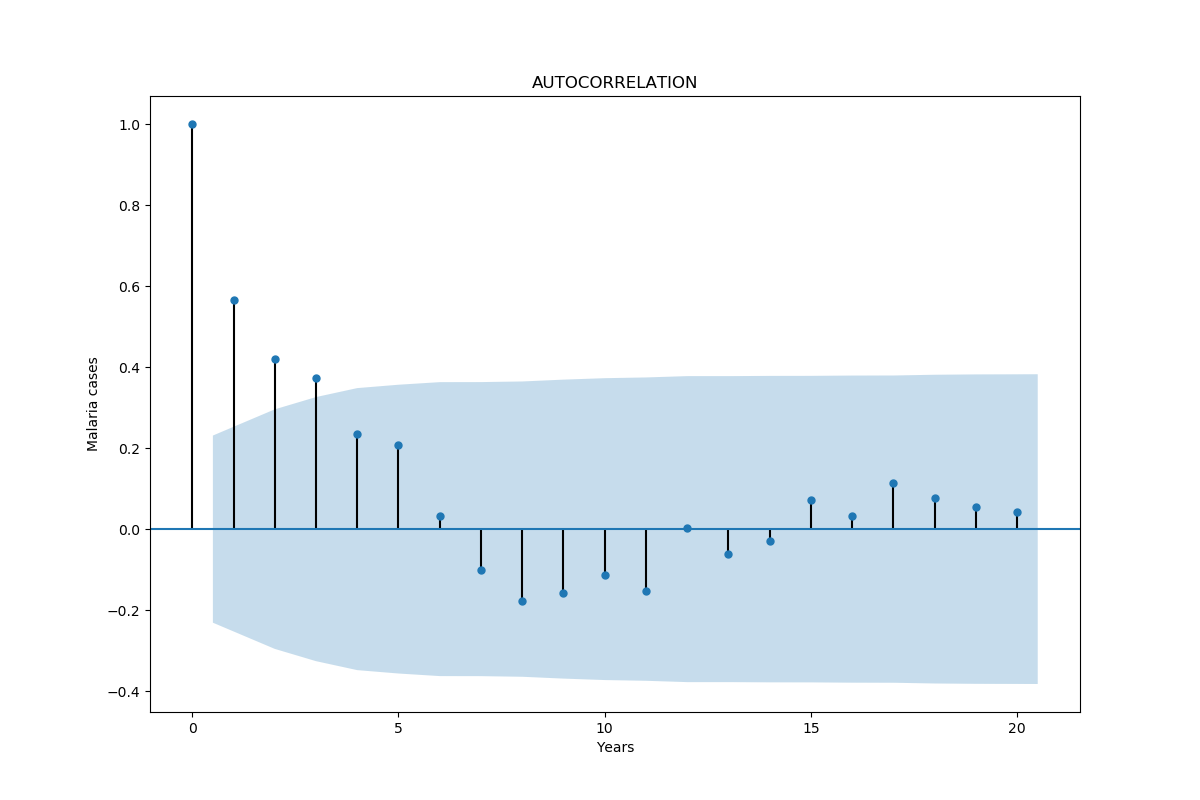
\includegraphics[scale=0.3]{MALARIA_DATA_ACF_PLOT.png}}
		    \caption{PLOTS FOR MALARIA DATA}
		        \label{fig:3}

\end{figure}
The Auto-correlation plot shows that there is autocorrelation at lag 1 as shown in the chart above. Therefore, a modified MannKendall test was used.\\   
Results from the Hamed and Rao Modified Mk test indicates that there is no trend in the malaria data set. A p-value of 0.3169 was obtained and this is higher than the 0.05. Therefore, we fail to reject the null hypothesis of no trend. 
\section{Conclusions}
pyMannKendall which is a python package can be used to determine trends in a data set. Three different data sets were used in this project. Results from the analysis indicates that the MannKendall Trend test can be used to determine whether there is a trend in a data set or not. Further, the issue of normality is not a problem when using the non-parametric pyMannKendall. 
\end{document}

